\newpage
\subsection{Caso d'uso UC10: Interazione Con API Registrate}
\label{UC10}
\begin{figure}[ht]
	\centering
	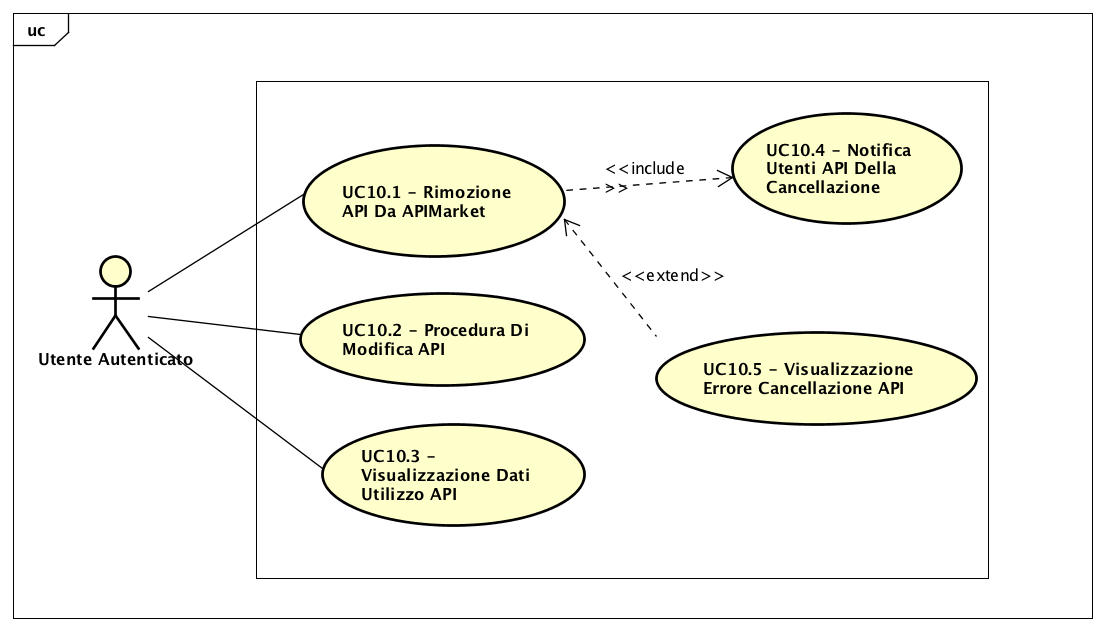
\includegraphics[scale=0.45]{UML/UC10.png}
	\caption{UC10: Interazione Con API Registrate}
\end{figure}

\renewcommand*{\arraystretch}{1.6}
\begin{longtable}{ l | p{11cm}}
	\hline
	\rowcolor{Gray}
	\multicolumn{2}{c}{UC10: Interazione Con API Registrate} \\
	\hline
	\textbf{Attori} &Utente Autenticato, Amministratore APIMarket, Interfacce API Presente In APIMarket \\
	\textbf{Descrizione} & l'attore sceglie attraverso quale modalità interagire con le API acquistate \\
	\textbf{Pre-Condizioni} & l'attore si trova nella schermata di gestione di una API acquistata\\
	\textbf{Post-Condizioni}&l'attore ha scelto l'interazione\\
	\textbf{Scenario Principale} & \begin{enumerate*}[label=(\arabic*.),itemjoin={\newline}]
			\item L'attore può rimuovere una propria API dall'APIMarket (UC10.1), inviando una notifica agli utenti di quella API (UC10.4);
		\item L'attore può modificare una propria API (UC10.2);
		\item L'attore può visualizzare i dati di utilizzo di una propria API (UC10.3);
	\end{enumerate*}\\
\end{longtable}



